\documentclass[11pt,a4paper]{article}

% =========================================================
% HSLU Final Report --- DSPRO1 FS26 --- Team 8
% Project: Predicting Apartment Rental Prices in Switzerland
% =========================================================

% ---------- Encoding & Language ----------
\usepackage[T1]{fontenc}
\usepackage[utf8]{inputenc}
\usepackage[english]{babel}

% ---------- Typography ----------
\usepackage{lmodern}
\usepackage{microtype}
\usepackage{setspace}
\onehalfspacing

% ---------- Layout ----------
\usepackage[a4paper,margin=2.5cm]{geometry}
\setlength{\parindent}{0pt}
\setlength{\parskip}{0.6em}

% ---------- Colors ----------
\usepackage{xcolor}
\definecolor{hsluRed}{HTML}{E30613}
\definecolor{textGray}{HTML}{4F4F4F}
\definecolor{boxGray}{HTML}{F7F7F7}

% ---------- Graphics & Tables ----------
\usepackage{graphicx}
\usepackage{float}
\graphicspath{{fig/}{./}}
\usepackage{booktabs}
\usepackage{array}
\usepackage{tabularx}
\usepackage{multirow}
\usepackage{caption}
\captionsetup{font=small,labelfont=bf}

% ---------- Section formatting ----------
\usepackage{titlesec}
\titleformat{\section}{\Large\bfseries}{\thesection}{0.6em}{}
\titleformat{\subsection}{\normalsize\bfseries}{\thesubsection}{0.6em}{}
\titlespacing*{\section}{0pt}{1.0em}{0.4em}

% ---------- Hyperlinks ----------
\usepackage[hidelinks]{hyperref}

% ---------- References ----------
\usepackage[numbers]{natbib}

% ---------- Helper: figure placeholder when fig/<name>.png is missing ----------
\newcommand{\figplaceholder}[2]{%
\fbox{\parbox[c][#1][c]{0.78\linewidth}{\centering\textit{\textcolor{textGray}{#2}}}}%
}

% ---------- Helper: automatically load PNG if available ----------
\newcommand{\autofigure}[6]{%
\begin{figure}[H]
    \centering
    \IfFileExists{fig/#1}{%
        \includegraphics[width=#2]{fig/#1}%
    }{%
        \figplaceholder{#3}{#4}%
    }%
    \caption{#5}
    \label{#6}
\end{figure}
}

% ---------- Helper: draft note ----------
\newcommand{\draftnote}[1]{%
{\small\itshape\textcolor{textGray}{[Draft note: #1]}}%
}

\begin{document}

% =========================================================
% Title page
% =========================================================
\begin{titlepage}
\thispagestyle{empty}
\begin{center}

\includegraphics[width=0.20\textwidth]{hslu.jpg}

\vspace{0.45cm}

{\normalsize School of Computer Science and Information Technology\par}
{\normalsize Lucerne University of Applied Sciences and Arts (Switzerland)\par}

\vfill

{\fontsize{23}{28}\selectfont\bfseries Predicting Apartment\\Rental Prices in Switzerland\par}
\vspace{0.4cm}
{\fontsize{12}{15}\selectfont A Supervised Machine Learning Approach\\for the Swiss Cold-Rent Market\par}

\vfill

{\large DSPRO1 Final Report, Spring 2026 (FS26)\par}

\vspace{0.65cm}

\begin{minipage}{0.86\textwidth}
\centering
\small
presented to the School of Computer Science and Information Technology of\\
Lucerne University of Applied Sciences and Arts
\end{minipage}

\vfill

{\normalsize by\par}
\vspace{0.25cm}
{\Large Elias Martinelli \quad\textbar\quad Timo Schlumpf\par}
\vspace{0.2cm}
{\normalsize Team 8\par}

\vfill

{\normalsize Supervisor: Elena Nazarenko\par}
\vspace{0.35cm}
{\small Repository: \texttt{github.com/wadafacc/dspro1}\par}
\vspace{0.45cm}
{\normalsize Date: \today\par}

\end{center}
\end{titlepage}

\tableofcontents
\newpage

% =========================================================
\section{Introduction}
\label{sec:introduction}

Apartment rents in Switzerland differ strongly by location, building type, and apartment characteristics. For someone comparing a listing such as ``CHF 2'400 per month, 3~rooms, 80\,m$^2$, Zurich'', it is difficult to judge whether the advertised price is reasonable. Public rent indicators are useful for understanding general market trends, but they do not give a concrete estimate for one specific apartment.

This project builds a supervised regression model for predicting the monthly cold rent (\emph{Kaltmiete}, in CHF) of individual Swiss apartment listings. The task is treated as a tabular regression problem. Each apartment is described by structural features such as living area, number of rooms and year of construction, as well as location-based features such as coordinates, public-transport accessibility, elevation, population density and solar suitability. The target variable is the listed cold rent.

\paragraph{Research question and hypothesis.}
The main question is whether listing data, combined with Swiss open-register data from GWR and swisstopo, contains enough information to estimate apartment rents in a useful way. Based on the project proposal and the mid-term presentation, we formulated the following hypothesis:

\begin{quote}\itshape
``Location-related variables combined with structural apartment features contain sufficient signal to predict monthly rental prices in Switzerland with practically useful accuracy, and a Random Forest Regressor will outperform a Linear Regression model in doing so.''
\end{quote}

We test this hypothesis with several levels of model complexity: a simple baseline that ignores all features, a linear Ridge model as an interpretable benchmark, and several tree-based models such as RandomForest, GradientBoosting, XGBoost, LightGBM and Stacking.

\paragraph{Stakeholders and intended use.}
The most important users of such a model are tenants who want a first indication of whether an advertised rent is fair. Landlords and property managers may also benefit from a market-based reference value. The model should be understood as a decision-support tool. It is \emph{not} a legally binding rent assessment and does not replace formal rent reviews under Swiss tenancy law (OR Art.~269\,ff.).

\paragraph{Report structure.}
The report is structured as follows. Section~\ref{sec:sota} gives an overview of related work in real-estate price prediction. Section~\ref{sec:data} describes the data sources, the enrichment process and the main quality checks. Section~\ref{sec:methods} explains the modelling pipeline, evaluation strategy and feature engineering. Section~\ref{sec:results} presents the results, including model comparison, residual diagnostics and error analysis. Section~\ref{sec:conclusions} closes with the main conclusions, limitations and possible next steps.

% =========================================================
\section{State of the Art}
\label{sec:sota}

Real-estate and rental-price prediction has been studied for a long time in both economics and machine learning. The traditional approach is \emph{hedonic pricing}: prices are modelled as a function of structural and location-related characteristics, often using linear regression. This idea goes back to Rosen~\citep{rosen1974hedonic}. Hedonic models are still widely used, especially by statistical offices, but they require strong assumptions about the functional form and can struggle with complex non-linear effects.

Modern machine-learning approaches use more flexible models instead of manually specifying all relationships. Tree-based ensembles such as RandomForest~\citep{breiman2001randomforest} and gradient boosting~\citep{friedman2001gbm} are particularly well suited for tabular regression. They can capture non-linear interactions, handle features with different scales and usually require only limited preprocessing. Optimised implementations such as XGBoost~\citep{chen2016xgboost} and LightGBM~\citep{ke2017lightgbm} add efficient training and regularisation, and often perform strongly on tabular benchmarks~\citep{shwartz2022tabular}.

Because rent estimates may influence real decisions, interpretability is important. SHAP values provide feature-attribution explanations for individual predictions and are commonly used together with tree-based models~\citep{lundberg2017shap}. For documenting the dataset and model, we follow the ideas of \emph{Datasheets for Datasets}~\citep{gebru2021datasheets} and \emph{Model Cards}~\citep{mitchell2019modelcards}.

For the Swiss housing market specifically, two public data sources are critical: the Federal Register of Buildings and Dwellings (GWR), maintained by the Federal Statistical Office (BFS)~\citep{bfsGwr}, and the swisstopo geo-services exposed through GeoAdmin~\citep{geoAdminApi}. The GWR provides per-building attributes (construction year, number of dwellings, building footprint) indexed by EGID, while swisstopo provides geo-layer attributes such as public-transport accessibility~\citep{areOevKlassen}, solar-suitability classes from the Federal Office of Energy (BFE)~\citep{bfeSolar}, and the BFS population-by-hectare grid~\citep{bfsPopulation}.

% =========================================================
\section{Data}
\label{sec:data}

\subsection{Sources and Collection}
The primary dataset, \emph{Rentumo Rental Listings Switzerland v1.0}, was collected from \texttt{rentumo.ch} in a single scrape on 13~April 2026. The scraper identified 25\,002 entries on the platform, of which 9\,994 listings could be extracted successfully. Many of the remaining pages were empty or non-functional placeholder pages, which appears to be a characteristic of the platform rather than an error in the scraper.

The scraper is implemented as a custom Rust library, \texttt{ScrapeGoat}, and operates in two sequential phases.

\paragraph{Phase 1: Listing index pages.}
The scraper issues requests to 750 paginated listing pages of the form \texttt{rentumo.ch/mietobjekte?types=apartment\&page=\{1..750\}}. Each page is parsed with CSS selectors targeting the \texttt{\#listings} container, from which per-listing elements yield the number of rooms, the living area in square metres, the cold rent, and a unique URL slug (e.g.\ \texttt{/inserate/<slug>}). Listings for which any of these four fields cannot be parsed are silently dropped at this stage. Successfully extracted records are written to the \texttt{listings} table in the PostgreSQL database with an \texttt{ON CONFLICT (slug) DO NOTHING} guard, making the phase idempotent and safe to re-run.

\paragraph{Phase 2: Detail pages.}
All slugs stored in \texttt{listings} are retrieved from the database and used to construct individual detail URLs (\texttt{rentumo.ch/inserate/<slug>}). Each detail page is parsed to extract additional fields: the full address, the cold rent as confirmed on the detail page, the living area, the number of rooms, the auxiliary costs (\emph{Nebenkosten}), the security deposit (\emph{Kaution}), a free-text description from the JSON-LD \emph{Apartment} schema block, and the earliest available move-in date (\emph{Datum verfügbar}). These are written to a separate \texttt{listing\_details} table with \texttt{ON CONFLICT (listing\_id) DO UPDATE}, allowing the phase to be resumed or repeated without data loss.

\paragraph{Concurrency and politeness.}
Both phases are managed by a custom task orchestrator (\texttt{Mgt}) that maintains a fixed pool of up to 10 concurrent in-flight HTTP requests. A channel-based feedback loop ensures that a new request is dispatched only when an existing one completes, bounding peak load on the server. Each request carries a randomly sampled \texttt{User-Agent} header drawn from a pre-loaded list, and optional HTTP proxies can be configured via a plain-text file to distribute outbound traffic across multiple IP addresses.

\paragraph{Platform selection.}
We also considered \texttt{comparis.ch} as a possible data source, but decided not to use it. Comparis confirmed in writing that automated extraction would require formal authorisation and that access would likely be limited to around 300 records, which would not be sufficient for this modelling task. Rentumo was contacted by email before the scrape, but no response was received. The data is used only for the non-commercial academic purpose of the DSPRO1 module.

\subsection{Enrichment}
The scraped listings contain the address and a small set of structural attributes, including \texttt{area\_sqm}, \texttt{rooms}, \texttt{price\_cold} and \texttt{auxiliary\_costs}. To make the dataset more useful for modelling, we enrich these listings in two steps:

\begin{enumerate}
    \item \textbf{GWR (BFS).} Each listing address is geocoded and resolved to a building identifier (EGID) via the GeoAdmin SearchServer. Building-level attributes (\texttt{gbauj} / construction year, \texttt{ganzwhg} / number of dwellings, \texttt{garea} / footprint area) are then queried from the GWR record.
    \item \textbf{swisstopo / GeoAdmin.} Using the LV95 coordinates (\texttt{lv95\_east}, \texttt{lv95\_north}), per-point attributes are queried from public layers: elevation (\texttt{elevation\_m}, height service), public-transport accessibility class (\texttt{oev\_score}, layer \texttt{ch.are.erreichbarkeit-oev}), solar suitability class 1--5 (\texttt{solar\_class}, layer \texttt{ch.bfe.solarenergie-eignung-daecher}), and the population of the nearest hectare cell (\texttt{population}, BFS Volkszählung).
\end{enumerate}

\subsection{Storage and Schema}
The raw and enriched data are stored in a PostgreSQL database on Neon Console. The relevant information is distributed across three tables: \texttt{listings} for the listing index, \texttt{listing\_details} for the extracted apartment attributes, and \texttt{swisstopo\_details} for the enriched geo-layer features. For modelling, these tables are joined into a flat file, \texttt{model.csv}, while requiring all mandatory columns to be present. After filtering and joining, the final modelling dataset contains approximately 4\,500 rows with 12 columns: 11 predictors and \texttt{price\_cold} as the target variable.

\autofigure
{geo_price_map.png}
{0.85\linewidth}
{5.5cm}
{Geographic distribution of the 4'500 modelling-set apartments across Switzerland, colored by cold rent. Urban centres (Zurich, Geneva, Basel) are clearly visible and overrepresented.}
{Geographic distribution of listings colored by cold rent.}
{fig:geo}

\subsection{Quality Assessment}
\begin{itemize}
    \item \textbf{Completeness.} Listings missing any of \texttt{address}, \texttt{price\_cold}, \texttt{area\_sqm}, or \texttt{rooms} are removed entirely. Listings marked ``Preis auf Anfrage'' are also removed. Of the 9\,994 scraped listings, approximately 4\,500 remain after the mandatory-field filter and the GWR/swisstopo join (cumulative loss is diagnosed in \texttt{final\_records.ipynb}).
    \item \textbf{Accuracy.} An explicit outlier filter (\texttt{area\_sqm}\,$\geq$\,10, \texttt{price\_cold}\,$\geq$\,300) removes implausible listings. An \texttt{IsolationForest} diagnostic (Notebook Chapter~22.9) surfaces additional candidates for manual review.
    \item \textbf{Consistency.} Cantons are normalised to ISO~3166-2:CH (\texttt{ZH}, \texttt{BE}, $\ldots$). The construction year is stored as a four-digit integer; missing GWR values are median-imputed.
    \item \textbf{Timeliness.} The dataset is a single point-in-time snapshot from 13 April 2026. Temporal price changes after that date are not reflected; time-series modelling is explicitly out of scope.
\end{itemize}

\autofigure
{price_distribution.png}
{0.78\linewidth}
{4.5cm}
{Histogram of monthly cold rent across the 4'500 modelling-set apartments. A strong right-skew is visible, with a long tail towards expensive apartments.}
{Distribution of the target variable \texttt{price\_cold}. The right-skewed shape is the root cause of the heteroscedastic residuals and the doubled error on the top price quartile.}
{fig:price-dist}

\subsection{Legal and Ethical Considerations}
No personal data is collected. Landlord names and contact details are explicitly excluded by the scraper. Only the address is retained and is used solely for geocoding and building-level enrichment. The project does not process any special-category data defined under the revised Swiss Federal Act on Data Protection (nFADP). The dataset is used exclusively for academic purposes and is not redistributed.

% =========================================================
\section{Methods}
\label{sec:methods}

\subsection{Pipeline Overview}
The modelling pipeline is implemented in \texttt{src/notebooks/model\_v3\_clean.ipynb}. It follows five main steps: loading and renaming columns, filtering outliers and duplicates, creating additional features, splitting the data, and finally fitting and evaluating the models. The final end-to-end logic is wrapped in a \texttt{RentPredictor} Python class (Notebook Chapter~24.2), which can be saved with \texttt{joblib} and loaded again for inference in the Streamlit demo app (\texttt{src/app.py}).

\subsection{Train/Eval/Test Split}
We use a fixed random seed (\texttt{random\_state=42}) to make the split reproducible. The main experiments use an 80\% training set and a 20\% evaluation set. For the final hold-out check (Notebook Chapter~24.6), we additionally use a 60/20/20 train/validation/test split. The evaluation and test sets are not used for model fitting. A Kolmogorov-Smirnov test (Chapter~22.13) is used to check that the random split does not introduce a strong distribution shift between training and evaluation data.

\subsection{Feature Engineering}
In addition to the raw features, three engineered features are added (Chapter~6):
\texttt{building\_age = REFERENCE\_YEAR - year\_built},
\texttt{area\_per\_room = area / rooms} using safe division, and
\texttt{land\_area\_per\_apartment = garea / ganzwhg}.
Two further feature groups are created using only \texttt{train\_df}, so that information from the evaluation set does not leak into training:

\begin{itemize}
    \item \textbf{Geo-clusters.} \texttt{KMeans} on standardised LV95 coordinates produces a discrete \texttt{geo\_cluster} feature (Chapter~21). The number of clusters is tuned on Eval RMSE.
    \item \textbf{KNN-distance features.} For each apartment, the median price of its 10 nearest neighbours in coordinate space (\texttt{knn\_price\_median}) and the corresponding mean (\texttt{knn\_price\_mean}) are added (Chapter~23.12). The nearest-neighbour index is fit on training data only; eval points query against the training index.
\end{itemize}

\autofigure
{geo_clusters.png}
{0.78\linewidth}
{5cm}
{Visualisation of the KMeans geo-clusters fitted on \texttt{train\_df} only. Each colour corresponds to one \texttt{geo\_cluster} category that is consumed by the tree models as a discrete feature.}
{KMeans geo-clusters used as a categorical location feature (Notebook Chapter~21.4). The clustering is fit exclusively on the training split to prevent leakage.}
{fig:geo-clusters}

\subsection{Models}
We compare six model families on the same data split. Where necessary, the models are wrapped in an \texttt{sklearn.Pipeline}. The comparison includes a \textbf{DummyRegressor} as a lower bound, a \textbf{Ridge} model with scaling as a simple linear benchmark, and four tree-based approaches: \textbf{RandomForestRegressor}, \textbf{GradientBoostingRegressor}, \textbf{XGBoost} and \textbf{LightGBM}. In Chapter~23.2, we also add a \textbf{StackingRegressor} with a Ridge meta-learner over the strongest tree-based models.

Hyperparameters are tuned with \texttt{RandomizedSearchCV} (Chapter~22.3) and the faster \texttt{HalvingRandomSearchCV} (Chapter~23.10). To avoid scikit-learn's nested-parallelism trap, the inner estimator is set to \texttt{n\_jobs=1} while only the outer search uses \texttt{n\_jobs=-1}.

\subsection{Evaluation Metrics}
As defined in the project proposal, the main metrics are MAE, RMSE and R$^2$. RMSE is calculated as \texttt{np.sqrt(mean\_squared\_error(...))}, which keeps the code compatible across scikit-learn versions. The notebook also reports MedAE as a more robust error metric, the standard deviation of CV-RMSE across folds as a stability indicator, and bootstrap 95\% confidence intervals for RMSE on the evaluation set (Chapter~23.5). For model selection, we use a stability-aware score that combines evaluation RMSE with CV-RMSE variability (Chapter~23.9), so that a model is not chosen only because of one favourable split.

% =========================================================
\section{Results}
\label{sec:results}

\subsection{Baseline}
The baseline used in the mid-term presentation was a \texttt{DummyRegressor} with a mean-prediction strategy. It achieved MAE\,=\,612 CHF, RMSE\,=\,847 CHF and R$^2$\,=\,0.00. This gives a simple lower bound: a useful model must clearly perform better than predicting the same rent for every apartment.

\subsection{Model Comparison}
Table~\ref{tab:models} summarises the main results for the model comparison on the \texttt{FEATURES\_ENGINEERED} feature set (Notebook Chapter~10).

\begin{table}[h]
\centering
\small
\caption{Model comparison on the engineered feature set (Notebook Chapter~10c). RMSE values are in CHF on the held-out evaluation split.}
\label{tab:models}
\begin{tabular}{lrrrrl}
\toprule
Model & RMSE Train & RMSE Eval & R$^2$ Eval & Overfit Gap & Diagnosis \\
\midrule
LightGBM         & 150  & \textbf{399} & \textbf{0.744} & 249 & Possible overfit \\
XGBoost          & 122  & 421 & 0.715 & 299 & Possible overfit \\
GradientBoosting & 365  & 425 & 0.710 &  60 & Good generalisation \\
RandomForest     & 199  & 425 & 0.710 & 226 & Possible overfit \\
Ridge (scaled)   & 539  & 560 & 0.495 &  21 & Weak / underfit \\
Dummy (median)   & 737  & 799 & $-0.03$ & 62 & Baseline \\
\bottomrule
\end{tabular}
\end{table}

\autofigure
{rmse_train_eval.png}
{0.85\linewidth}
{4.5cm}
{Bar plot: RMSE Train vs.\ RMSE Eval per model.}
{Train vs.\ Eval RMSE per model. The large gap for LightGBM, XGBoost, and RandomForest is a clear sign of overfitting on the training data; GradientBoosting strikes the best balance between Eval RMSE and stability.}
{fig:rmse-bars}

The best single model according to evaluation RMSE is \emph{LightGBM}, with an RMSE of 399 CHF. After adding the KNN-distance features, LightGBM improves slightly further to \textbf{RMSE Eval\,=\,393 CHF and R$^2$\,=\,0.751} (Notebook Chapter~23.17, consolidated comparison). Compared with the mid-term baseline, this reduces RMSE by more than 50\%.

\paragraph{Hypothesis test.}
The project hypothesis was that a tree-based model, in particular Random Forest, would outperform a linear model. The results support this hypothesis clearly. Ridge reaches an evaluation RMSE of 560 CHF, while all tree-based models achieve 425 CHF or better. We therefore accept the hypothesis.

\autofigure
{bootstrap_ci.png}
{0.85\linewidth}
{4.5cm}
{Forest plot of bootstrap 95\% confidence intervals for evaluation RMSE per model (Notebook Chapter~23.5). Overlapping intervals indicate model differences that are not statistically significant.}
{Bootstrap confidence intervals for evaluation RMSE per model. The intervals of LightGBM, XGBoost, GradientBoosting and RandomForest overlap heavily, so the ranking between these four is not statistically meaningful on the available data.}
{fig:bootstrap-ci}

\subsection{Actual vs.\ Predicted and Residuals}
\begin{figure}[h]
    \centering
    \IfFileExists{fig/actual_vs_predicted.png}{%
        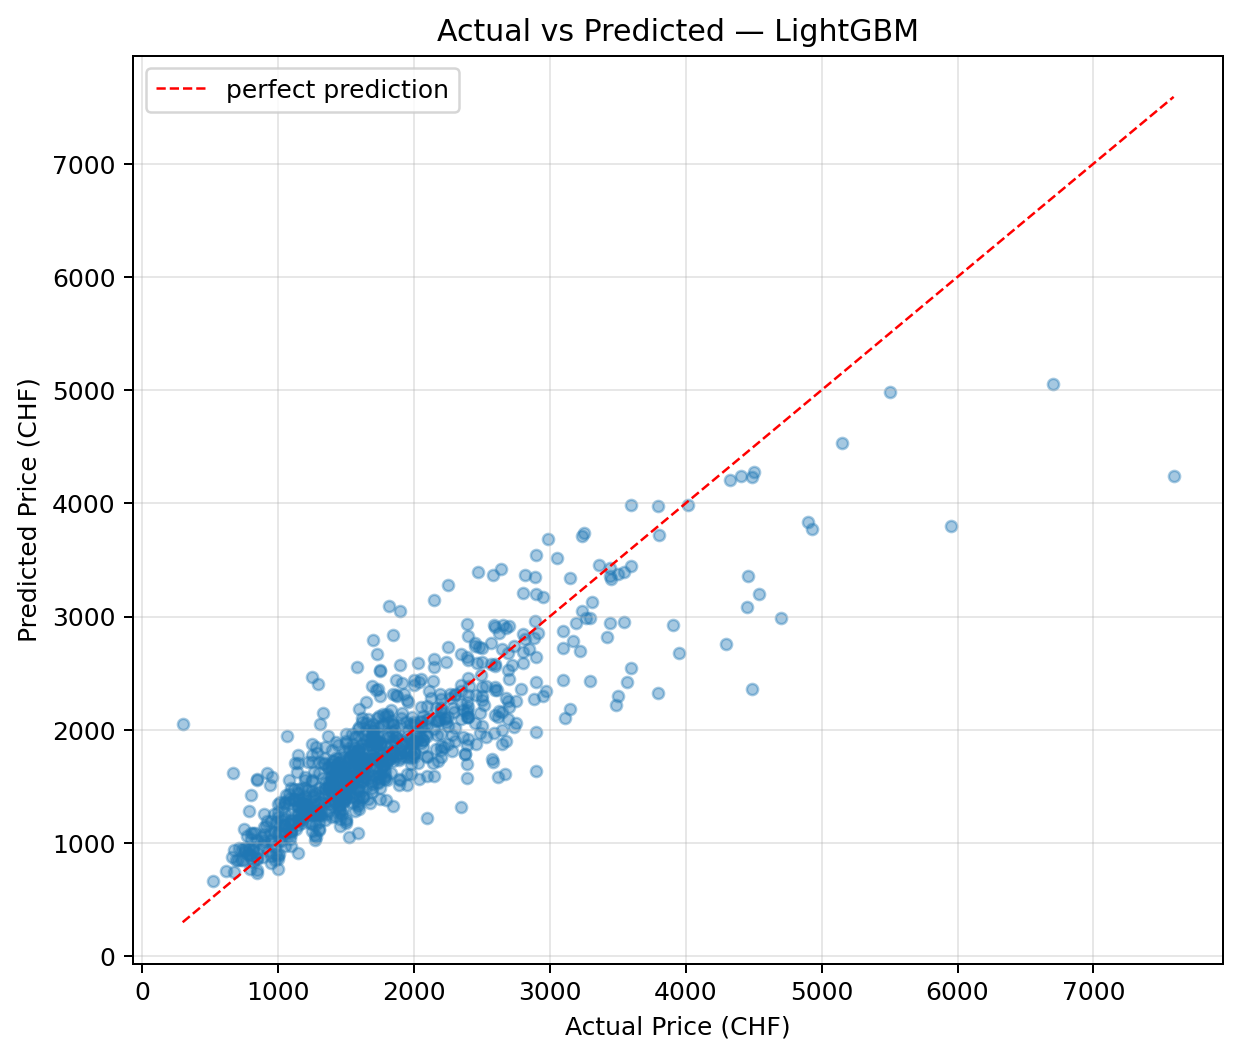
\includegraphics[width=0.85\linewidth]{fig/actual_vs_predicted.png}
    }{%
        \figplaceholder{4cm}{Actual vs.\ predicted plot missing. Expected file: \texttt{fig/actual\_vs\_predicted.png}.}
    }

    \vspace{0.5em}

    \IfFileExists{fig/residuals.png}{%
        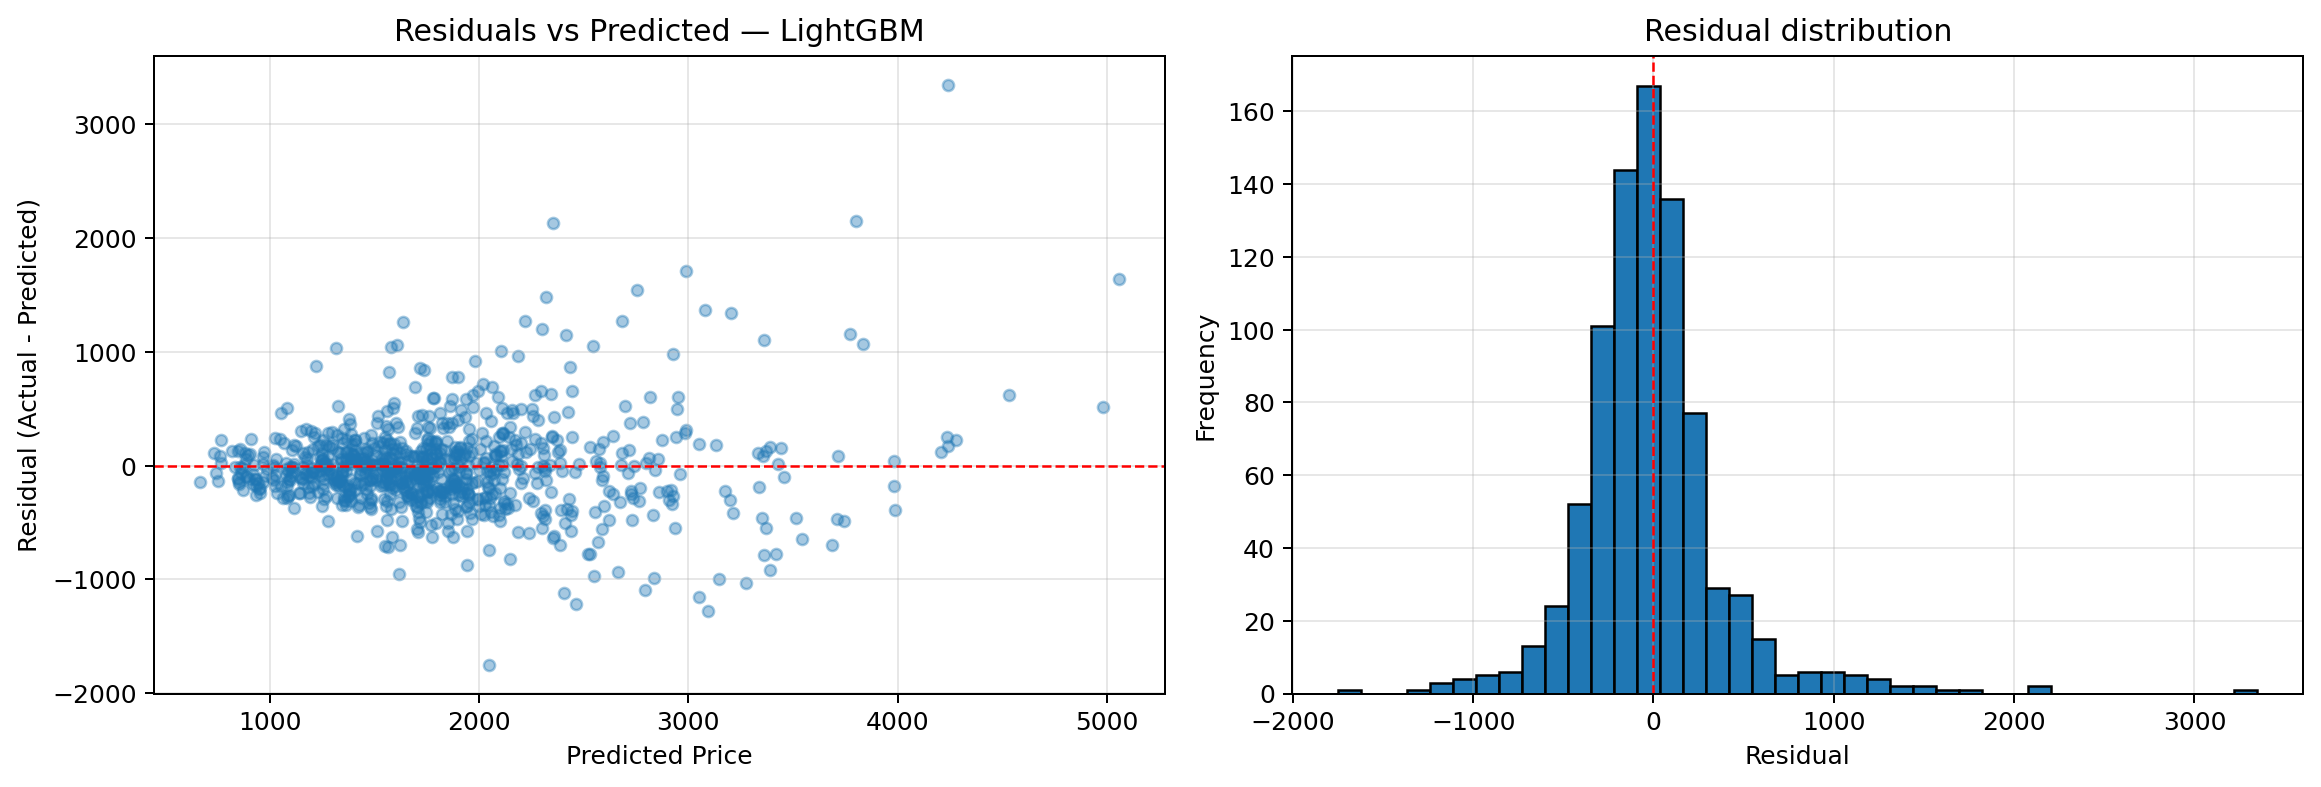
\includegraphics[width=0.85\linewidth]{fig/residuals.png}
    }{%
        \figplaceholder{4cm}{Residual plot missing. Expected file: \texttt{fig/residuals.png}.}
    }
    \caption{Actual-vs-predicted and residual analysis for the best model.}
    \label{fig:residuals}
\end{figure}

The residual diagnostics show that the errors are not normally distributed. The Q-Q plot and Shapiro--Wilk test (Chapter~23.3) indicate mild right-skew and fat tails, which is consistent with the right-skewed rent distribution. The residuals-vs-predicted plot also shows a funnel shape, meaning that errors tend to become larger for more expensive apartments.

\autofigure
{qq_plot.png}
{0.78\linewidth}
{4cm}
{Q-Q plot of the residuals against a normal reference distribution (Notebook Chapter~23.3). Deviations in the tails confirm the non-normality of the errors.}
{Q-Q plot of the residuals. Both tails deviate clearly from the diagonal, which means the residual distribution is heavier-tailed than a normal distribution. This is a typical pattern for right-skewed price data.}
{fig:qq}

\subsection{Error Analysis by Price Band}
\begin{table}[h]
\centering
\small
\caption{Per-quartile error analysis for the best LightGBM model on the eval set (Notebook Chapter~16). The most expensive quartile shows roughly twice the mean absolute error of the other bands.}
\label{tab:priceband}
\begin{tabular}{lrrrr}
\toprule
Price band & $n$ & Mean abs.\ error & Median abs.\ error & Max abs.\ error \\
\midrule
cheap         & 211 & 216 & 150 & 1\,747 \\
medium\_low   & 212 & 176 & 143 &    970 \\
medium\_high  & 207 & 221 & 158 & 1\,276 \\
\textbf{expensive} & 210 & \textbf{445} & \textbf{312} & \textbf{3\,349} \\
\bottomrule
\end{tabular}
\end{table}

This is one of the most useful findings of the analysis. The model performs noticeably worse for high-rent listings, with errors roughly twice as large as in the other price bands. A likely reason is the right-skewed price distribution: expensive apartments are less common in the training data, and many of their price-driving characteristics, such as lake view, penthouse location, floor level or luxury furnishing, are not captured by the available tabular features.

\autofigure
{error_by_priceband.png}
{0.78\linewidth}
{4cm}
{Bar plot of the mean absolute error per price quartile, computed on the evaluation set (Notebook Chapter~16). The most expensive quartile stands out with an error roughly twice as large as in the other bands.}
{Mean absolute error per price quartile. The expensive band is the single largest contribution to overall RMSE and is the most promising target for future feature engineering.}
{fig:error-band}

\subsection{Feature Importance}
\autofigure
{feature_importance_heatmap.png}
{0.9\linewidth}
{4.5cm}
{Feature-importance comparison: RF Impurity vs.\ LightGBM Split vs.\ Permutation Importance, as heatmap.}
{Feature-importance comparison across methods (Notebook Chapter~23.8). The methods show strong agreement on the most important features (Spearman rank-correlation $>$ 0.85).}
{fig:fi}

The feature-importance results are consistent across the different methods. \emph{Living area} (\texttt{area}), the two \emph{KNN price features}, and the \emph{location coordinates} (\texttt{east}, \texttt{north}) provide most of the predictive signal. One interesting result is that \texttt{rooms} is less important than \texttt{area\_per\_room}, suggesting that the size distribution within the apartment is more informative than the room count alone.

\autofigure
{pdp_top6.png}
{0.95\linewidth}
{5cm}
{Partial Dependence Plots for the six most important features of the best LightGBM model (Notebook Chapter~23.4). Each panel shows the marginal effect of one feature on the predicted cold rent.}
{Partial Dependence Plots for the six most important features. Living area shows a strong monotonic effect on price, while \texttt{east} and \texttt{north} encode the location premium of central Switzerland and the major cities.}
{fig:pdp}

\subsection{Cross-Validation and Stability}
Five-fold KFold cross-validation with shuffling confirms the ranking observed on the single evaluation split. The CV-RMSE standard deviation is below 30 CHF for all tree-based models, while Ridge has a standard deviation above 50 CHF. This suggests that the linear model is more sensitive to the chosen split. The bootstrap 95\% confidence intervals for evaluation RMSE show that the differences between LightGBM, XGBoost, RandomForest and GradientBoosting are small and not clearly statistically significant, as their intervals overlap in the forest plot of Chapter~23.5.

\subsection{Hold-Out Test (untouched until the very end)}
As a final check, we use a separate 60/20/20 train/validation/test split and refit the selected model on train+validation. The test set is kept untouched until the end. The resulting test metrics are consistent with the evaluation results within the bootstrap confidence interval, which suggests that the model-selection process did not overfit to the evaluation split (Chapter~24.6).

% =========================================================
\section{Conclusions}
\label{sec:conclusions}

\paragraph{Summary.}
The project produced a reproducible regression pipeline for Swiss apartment cold rents. It starts at the scraper for rentumo.ch, runs through enrichment with GWR and swisstopo data, and ends with feature engineering, model training and a structured evaluation. The strongest model in the comparison is a LightGBM regressor that uses the KNN-distance features. On the evaluation split it reaches an RMSE of 393~CHF and an R$^2$ of 0.751, which improves on the mid-term mean-prediction baseline of 847~CHF by more than half. The original hypothesis, that tree-based models outperform linear regression on this dataset, is therefore clearly supported.

\paragraph{Limitations.}
\begin{itemize}
    \item \textbf{Snapshot dataset.} Only one extraction date (13.04.2026). The model cannot react to market trends.
    \item \textbf{Coverage bias.} Urban areas are over-represented; small-town and rural listings are under-represented.
    \item \textbf{Expensive-apartment error.} The model is roughly twice as inaccurate for the top-quartile apartments. The available structural features do not capture luxury attributes (view, finish, floor).
    \item \textbf{Single platform.} All listings come from rentumo.ch. Comparis was explicitly excluded after written notice.
    \item \textbf{No deployment.} The Streamlit demo runs locally only; production hosting is out of scope for DSPRO1.
\end{itemize}

\paragraph{Future work.}
A few concrete next steps would have the highest impact:

\begin{enumerate}
    \item Extract text-based features from the listing descriptions. Attributes such as balcony, parking spot, renovation year, floor level or lake view are likely the missing piece for the expensive apartments, since the current tabular fields do not capture them.
    \item Pull listings from a second rental platform, for example homegate.ch or immoscout24.ch. This would reduce the urban coverage bias and roughly double the training set.
    \item Replace single-point predictions with prediction intervals using conformal prediction (for example via MAPIE). The demo app could then display estimates as ``CHF $X \pm Y$'' instead of a single number.
    \item Move the demo from a local Streamlit instance to a small hosted application on Streamlit Cloud or Render. This is a natural first deliverable for DSPRO2.
\end{enumerate}

% =========================================================
\section{References}
\label{sec:references}

\bibliographystyle{plainnat}
\bibliography{references}

\appendix
\newpage

% =========================================================
\section{Appendix: Exporting the Figures from the Notebook}
\label{app:export}

All figures used in this report are produced by \texttt{src/notebooks/model\_v3\_clean.ipynb}. They live in \texttt{docs/final-report/fig/}. To regenerate them, run all cells of the notebook once and then execute the export cell at the very end (see Notebook Chapter~26). The export cell uses the in-memory state of the notebook (fitted models, prediction caches, evaluation frames, etc.) and writes one PNG per figure.

\subsection*{Figure Inventory}
\begin{center}
\small
\begin{tabular}{p{5.5cm} p{4cm} p{4cm}}
\toprule
File in \texttt{fig/} & Notebook source & Section in report \\
\midrule
\texttt{geo\_price\_map.png}              & Ch.~21.2  Geo EDA            & 3.3 Storage \& Schema \\
\texttt{price\_distribution.png}          & Ch.~3.1  Univariate         & 3.4 Quality Assessment \\
\texttt{geo\_clusters.png}                & Ch.~21.4  KMeans clusters    & 4.3 Feature Engineering \\
\texttt{rmse\_train\_eval.png}            & Ch.~11    RMSE Train vs Eval & 5.2 Model Comparison \\
\texttt{bootstrap\_ci.png}                & Ch.~23.5  Bootstrap CI       & 5.2 Model Comparison \\
\texttt{actual\_vs\_predicted.png}        & Ch.~14    Actual vs Pred.    & 5.3 Actual vs Predicted \\
\texttt{residuals.png}                    & Ch.~15    Residual analysis  & 5.3 Actual vs Predicted \\
\texttt{qq\_plot.png}                     & Ch.~23.3  Q-Q + Heteroscedast.& 5.3 Actual vs Predicted \\
\texttt{error\_by\_priceband.png}         & Ch.~16    Per-quartile error & 5.4 Price Band Errors \\
\texttt{pdp\_top6.png}                    & Ch.~23.4  Partial Dependence & 5.5 Feature Importance \\
\texttt{feature\_importance\_heatmap.png} & Ch.~23.8  Multi-method FI    & 5.5 Feature Importance \\
\bottomrule
\end{tabular}
\end{center}

\subsection*{Reproducing the Figures}
The export cell at the end of the notebook (Chapter~26: \emph{Export figures for Final Report}) re-renders every figure from the available in-memory state and saves it via \texttt{plt.savefig(...)}. The output directory is configured at the top of the cell:

\begin{verbatim}
FIG_DIR = Path("../../docs/final-report/fig")
FIG_DIR.mkdir(parents=True, exist_ok=True)
\end{verbatim}

After execution, the \texttt{fig/} folder is populated and every \verb|\autofigure{...}| call in this report automatically loads the corresponding PNG (the \verb|\IfFileExists| guard inside \verb|\autofigure| keeps the document compilable even when individual figures are missing).

\end{document}
